\documentclass[letterpaper,10pt,titlepage, onecolumn, draftclsnofoot]{IEEEtran}

\usepackage{graphicx}                                     
\usepackage{amssymb}                                       
\usepackage{amsmath}                                       
\usepackage{amsthm}  
\usepackage{sectsty}
\usepackage{alltt}                                         
\usepackage{float}
\usepackage{color}
\usepackage{url}

\usepackage{balance}
\usepackage[TABBOTCAP, tight]{subfigure}
\usepackage{enumitem}
\usepackage{pstricks, pst-node}

\usepackage{geometry}
\geometry{textheight=8.5in, textwidth=6in}

\newcommand{\cred}[1]{{\color{red}#1}}
\newcommand{\cblue}[1]{{\color{blue}#1}}

\usepackage{hyperref}
\usepackage{geometry}

\hypersetup{
  colorlinks = true,
  urlcolor = black,
  pdfauthor = {\name},
  pdfkeywords = {CS461 ``Senior Software Engr Project'' User Requirement},
  pdftitle = {CS 461 User Requirement},
  pdfsubject = {CS 461 User Requirement},
  pdfpagemode = UseNone
}

\begin{document}
\begin{titlepage}
\begin{center}
  
  \textbf{}

  \vspace{4cm}
  \Huge{}
  User Requirement
  \vspace{1.5cm}

 
  \LARGE
  CS461 - Senior Software Engr Project\\
  \vspace{0.25cm}
  Instructor: D. Kevin McGrath \\
  Instructor: Kristen Winters \\
  \vspace{0.25cm}
  Fall 2018 \\
  \vspace{1.5cm}
  
  \large{Bhavya Parikh, Davian Lukman, Eli Laudi, Matthew L. Jansen, and Ryan Sisco}\\
  \date{October 18th, 2018}
  \vfill
  November 6th, 2018\\
  \vspace{1cm}
  \vspace*{\fill}

   \normalsize 
\end{center}
\end{titlepage}
  
\section{Introduction}
\noindent This document will discuss in depth the system requirements for the 3D Visualization project. We will examine the purpose and scope of the project, and define the context and functionality of the system as a whole. 

    \subsection{System Purpose}
    \noindent The purpose of this system is to generate and populate a 3D representation of provided data. This is done to provide a better understanding of the collected information and group similarities in the file.

    \subsection{System Scope}
    \noindent The application that will be implemented to fix this problem will be "name". It will address the need for a simple tool that converts a universally accepted way of storing data, a CSV file, into an easily comprehensible 3D graph.

    \subsection{System Overview}
    \noindent "name" is a web app application that visualizes data in 3D. It provides tools to parse a CSV input file and render it in the form of 3D axes with charts and maps.
        \subsubsection{System Context}
        PC/Laptop
        \subsubsection{System Functions}
        Read from CSV file, Render 3D Data, Interact with 3D Data
        \subsubsection{User Characteristics}
        "name" can be run locally or hosted on a web server. This means that it is possible to only have one user who both launches the web app and uses it or have a user who accesses the web page and a person who maintains the web app.

    \subsection{Definitions, Acronyms, and Abbreviations}
    \noindent A CSV file is a comma separated value file. By mentioning CSV file, there will be rows and columns of data that the application could take. Any mention of 3D is referencing three dimensions. FPS is a measurement of frames per second, meaning how many times is an image displayed on a screen in a given second.

\section{System Requirement}
\noindent Here, we will define the system requirements which define the functional boundaries of our system. These will assist in characterizing the properties and behaviors of the system.

    \subsection{Functional Requirements}
    \begin{enumerate}
        \item The application shall be able to parse a CSV file.
        \item A 3D graphic display shall be provided based on CSV data.
        \item The 3D graphic shall respond to changes in data or constraints.
    \end{enumerate}
    
    \subsection{Usability Requirements}
    \begin{enumerate}
        \item The system shall provide the user with a method to upload a CSV file into the web application. 
        \item The system shall provide the user with a method to add, edit, and/or remove objects and relationships to the data before it is displayed in it's 3D environment.
        \item The system's display of data shall provide interactive possibilities for the user to engage with.
    \end{enumerate}
        
    \subsection{Performance Requirements}
    \begin{enumerate}
        \item The system should be able to handle large amounts of data.
        \item The rendering of the data should stay above 30 FPS for comfortable viewing.
    \end{enumerate}
    
    \subsection{System Interface}
    \noindent The system interface is a web application. It can be accessed via a browser such as Chrome, Firefox, etc.
 
 
\section{Assumptions and Dependencies}
\begin{enumerate}
    \item The CSV file the user uploads has at least 3 columns.
    \item System is error free.
    \item Assume the user is using a browser that supports the application.
\end{enumerate}
    
\section{Appendices}
    \subsection{Gantt Chart}
     \begin{figure}[H]
         \centering
                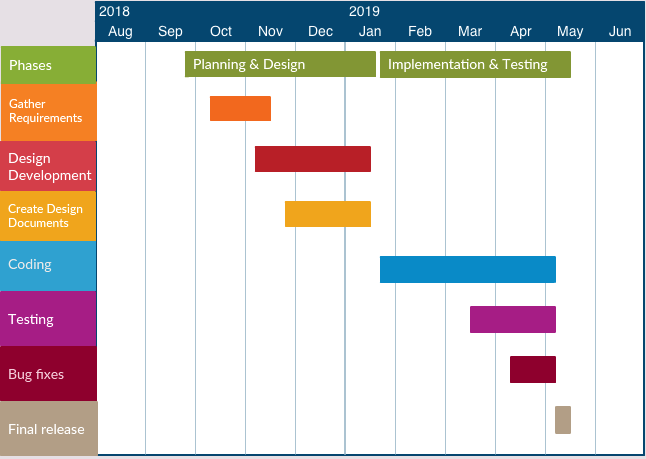
\includegraphics[width=\linewidth]{./image.png}
     \end{figure}
 
\newpage  



\end{document}